\documentclass{beamer}

\usepackage{amssymb,amsmath}
\usepackage{graphicx}
\usepackage{url}
\usepackage{color}
\usepackage{relsize}		% For \smaller
\usepackage{url}			% For \url
\usepackage{epstopdf}	% Included EPS files automatically converted to PDF to include with pdflatex

%For MindMaps
% \usepackage{tikz}%
% \usetikzlibrary{mindmap,trees,arrows}%

%%% Color Definitions %%%%%%%%%%%%%%%%%%%%%%%%%%%%%%%%%%%%%%%%%%%%%%%%%%%%%%%%%
%\definecolor{bordercol}{RGB}{40,40,40}
%\definecolor{headercol1}{RGB}{186,215,230}
%\definecolor{headercol2}{RGB}{80,80,80}
%\definecolor{headerfontcol}{RGB}{0,0,0}
%\definecolor{boxcolor}{RGB}{186,215,230}

%%% Save space in lists. Use this after the opening of the list %%%%%%%%%%%%%%%%
%\newcommand{\compresslist}{
%	\setlength{\itemsep}{1pt}
%	\setlength{\parskip}{0pt}
%	\setlength{\parsep}{0pt}
%}

%\setbeameroption{show notes on top}

% You should run 'pdflatex' TWICE, because of TOC issues.

% Rename this file.  A common temptation for first-time slide makers
% is to name it something like ``my_talk.tex'' or
% ``john_doe_talk.tex'' or even ``discrete_math_seminar_talk.tex''.
% You really won't like any of these titles the second time you give a
% talk.  Try naming your tex file something more descriptive, like
% ``riemann_hypothesis_short_proof_talk.tex''.  Even better (in case
% you recycle 99% of a talk, but still want to change a little, and
% retain copies of each), how about
% ``riemann_hypothesis_short_proof_MIT-Colloquium.2000-01-01.tex''?

\mode<presentation>
{
  % A tip: pick a theme you like first, and THEN modify the color theme, and then add math content.
  % Warsaw is the theme selected by default in Beamer's installation sample files.

  %%%%%%%%%%%%%%%%%%%%%%%%%%%% THEME
  %\usetheme{AnnArbor}
  %\usetheme{Antibes}
  %\usetheme{Bergen}
  %\usetheme{Berkeley}		% bem bacana - menu esquerdo
  %\usetheme{Berlin}
  %\usetheme{Boadilla}
  %\usetheme{boxes}
  %\usetheme{CambridgeUS}		% bem bacana - menu superior
  %\usetheme{Copenhagen}
  %\usetheme{Darmstadt}
  %\usetheme{default}
  %\usetheme{Dresden}
  \usetheme{Frankfurt}
  %\usetheme{Goettingen}
  %\usetheme{Hannover}		% bem bacana - menu esquerdo
  %\usetheme{Ilmenau}
  %\usetheme{JuanLesPins}
  %\usetheme{Luebeck}
  %\usetheme{Madrid}		%bacana
  %\usetheme{Malmoe}
  %\usetheme{Marburg}		% bem bacana - menu direito
  %\usetheme{Montpellier}
  %\usetheme{PaloAlto}		% bem bacana - menu esquerdo
  %\usetheme{Pittsburgh}
  %\usetheme{Rochester}		%bacana
  %\usetheme{Singapore}
  %\usetheme{Szeged}
  %\usetheme{Warsaw}

  %%%%%%%%%%%%%%%%%%%%%%%%%%%% COLOR THEME
  %\usecolortheme{albatross}		% azul escuro, massa
  %\usecolortheme{beetle}		% cinza, menu azul
  %\usecolortheme{crane}		% branco e amarelo, massa
  \usecolortheme{default}		% branco, azul clarinho
  %\usecolortheme{dolphin}		% azul e branco, legal
  %\usecolortheme{dove}			% cinza e branco, feio
  %\usecolortheme{fly}			% todo cinza, horrível
  %\usecolortheme{lily}			% parece o default
  %\usecolortheme{orchid}		% azul e branco, ok
  %\usecolortheme{rose}			% branco e violeta-claro, bonito
  %\usecolortheme{seagull}		% cinza, feio
  %\usecolortheme{seahorse}		% nhé, meio feio
  %\usecolortheme{sidebartab}		% Azul, branco, destaque na tab, interessante
  %\usecolortheme{structure}		% bichado
  %\usecolortheme{whale}		% Azul e branco, bem bonito

  %%%%%%%%%%%%%%%%%%%%%%%%%%%% OUTER THEME
  \useoutertheme{default}
  %\useoutertheme{infolines}
  %\useoutertheme{miniframes}
  %\useoutertheme{shadow}
  %\useoutertheme{sidebar}
  %\useoutertheme{smoothbars}
  %\useoutertheme{smoothtree}
  %\useoutertheme{split}
  %\useoutertheme{tree}

  %%%%%%%%%%%%%%%%%%%%%%%%%%%% INNER THEME
  \useinnertheme{circles}
  %\useinnertheme{default}
  %\useinnertheme{inmargin}
  %\useinnertheme{rectangles}
  %\useinnertheme{rounded}

  %%%%%%%%%%%%%%%%%%%%%%%%%%%%%%%%%%%

  \setbeamercovered{invisible} % or whatever (possibly just delete it)
  % To change behavior of \uncover from graying out to totally
  % invisible, can change \setbeamercovered to invisible instead of
  % transparent. apparently there are also 'dynamic' modes that make
  % the amount of graying depend on how long it'll take until the
  % thing is uncovered.

}


% Get rid of nav bar
\beamertemplatenavigationsymbolsempty

% Use short top
%\usepackage[headheight=12pt,footheight=12pt]{beamerthemeboxes}
%\addheadboxtemplate{\color{black}}{
%\hskip0.5cm
%\color{white}
%\insertshortauthor \ \ \ \ 
%\insertframenumber \ \ \ \ \ \ \ 
%\insertsection \ \ \ \ \ \ \ \ \ \ \ \ \ \ \ \ \  \insertsubsection
%\hskip0.5cm}
%\addheadboxtemplate{\color{black}}{
%\color{white}
%\ \ \ \ 
%\insertsection
%}
%\addheadboxtemplate{\color{black}}{
%\color{white}
%\ \ \ \ 
%\insertsubsection
%}

% Insert frame number at bottom of the page.
% \usefoottemplate{\hfil\tiny{\color{black!90}\insertframenumber}} 

\usepackage[english]{babel}
\usepackage[latin1]{inputenc}
\usepackage{subfigure}

\usepackage{times}
\usepackage[T1]{fontenc}


\title[GB21802]{GB21802 - Programming Challenges}
\subtitle[]{Week 3 - Dynamic Programming}
\author[Claus Aranha]{Claus Aranha\\{\footnotesize caranha@cs.tsukuba.ac.jp}}
\institute{College of Information Science}
\date{2019-05-10,13\\{\tiny Last updated \today}}

\begin{document}

\section{Introduction}
\subsection{Title}
\begin{frame}
\maketitle
\end{frame}

\subsection{Notes from Previous Classes}

\begin{frame}
  \frametitle{Results for the Previous Week}

  \begin{center}
    Here are the results for last week:

    \bigskip
    
    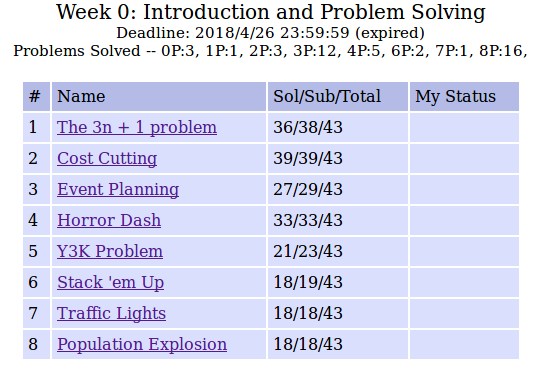
\includegraphics[width=0.8\textwidth]{img/resultW0}
    
    \bigskip

    Hope you enjoyed the warm up!
  \end{center}

\end{frame}

\begin{frame}[fragile]
  \frametitle{Comments from e-mails and questions -- 1}

  \begin{block}{Submission with Java}
    Two students had \structure{``runtime error''} with Java last week
    -- don't forget that your start class MUST be called {\bf Main}.
  \end{block}

  \vfill

\begin{verbatim}
class Main {
  public static void main(String[] args) {

    // do something...

  }
}
\end{verbatim}
\end{frame}

\begin{frame}
  \frametitle{Comments from e-mails and questions -- 2}
  \begin{block}{Input/Output}
    Two other students had problems because their program printed ``Please enter a number''.

    \bigskip

    You are very kind, but please {\bf follow the specifications} strictly!
  \end{block}
  
  \vfill

  \begin{block}{Format for MANABA submission}
    One student asked if the code for MANABA had to be the same as the code for UVA.

    \bigskip

    Yes. The code you submit on MANABA must be {\bf exactly the same}
    as the code you submitted for UVA.
  \end{block}
\end{frame}

\begin{frame}
  \frametitle{Short comments about the problems:}
  \begin{itemize}
  \item Cost Cutting, Event Planning, Horror Dash -- Easiest problems (find mean, find min, find min);
    \bigskip

  \item 3n+1 -- Still easy, but a few traps -- example of {\bf Memoization};
    \bigskip

  \item Y3K Problem -- Still easy, but skip year can be a bit troublesome.
    
  \end{itemize}
\end{frame}

%\begin{frame}
%  \frametitle{Comments about the problems}
%\end{frame}


\subsection{Outline}

\begin{frame}
  \frametitle{Quick Review of Last week}
  \begin{itemize}
  \item Definition of a \structure{Search Problem}
  \item Three types of algorithms for search problems:
    \begin{itemize}
    \item Complete Search
    \item Divide and Conquer
    \item Greedy Search
    \end{itemize}
  \end{itemize}

  \bigskip

  \begin{block}{}
    This week we introduce the last, and arguably most important
    algorithm for search problems: \structure{Dynamic Programming}
  \end{block}
\end{frame}

\subsection{Definition of Dynamic Programming}
\begin{frame}
  \frametitle{What is Dynamic Programming (DP)?}

  \structure{DP} is technique for \structure{Search Problems} which is
  based on the idea of \alert{building partial solutions}.

  \bigskip

  \begin{block}{Basic Idea of DP}
    Create a 2D table where:
    \begin{itemize}
    \item The rows are possible choices for the problem;
    \item The columns are sub-solutions for the problem;
    \end{itemize}

    \medskip
    First, fill the first column with each possible choice.\\

    \medskip

    Second, fill column n+1 with the combination of \structure{best
      solution for n and best choice for n+1|n}.
  \end{block}
\end{frame}

\begin{frame}
  \frametitle{Characteristics of DP:}

  \begin{block}{Used for \emph{optimization} or \emph{counting} problems}
    \begin{itemize}
    \item ``Count the number of solutions...''
    \item ``Find the minimum cost...''
    \item ``Find the maximum length...''
    \end{itemize}
  \end{block}

  \begin{exampleblock}{DP depends on \emph{number of states} and \emph{induction}}
      \begin{itemize}
      \item The \structure{complexity} of DP is based on the size of the table;
      \item The \structure{correctness} of DP is based on the idea of induction;
      \end{itemize}
  \end{exampleblock}
\end{frame}

\section{Initial Example}

\subsection{Introductory Problem: Wedding}

\begin{frame}
    \frametitle{Problem Example: Wedding Shopping -- UVA 11450}

    \begin{block}{}
      Best way to understand DP is to \structure{do a lot of examples!}
    \end{block}

    \vfill

    Buying problem:
    \begin{itemize}
    \item Buy one of each $C$ classes of items.
    \item Maximize the cost, but \structure{do not exceed the budget} $M$
    \end{itemize}

    \medskip

    \begin{columns}
      \column{0.7\textwidth}
      \begin{itemize}
      \item $M \leq 200$, $C \leq 20$;
      \item Each class has $0 < K_i \leq 20$ options;
      \item Total possible choices: $20^{20}$!
      \end{itemize}

      \column{0.3\textwidth}
      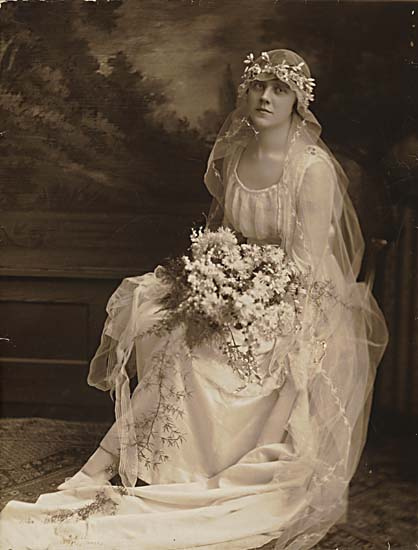
\includegraphics[width=.8\textwidth]{../img/weddingdress}\\
    \end{columns}
    \vfill
    {\tiny
    \hfill Image CC-By-2.0 by \url{https://www.flickr.com/photos/vancouver125/5634967507}}

\end{frame}

\begin{frame}
  \frametitle{Problem Example: Wedding Shopping -- UVA 11450}
  \begin{block}{Sample case 1: $C=3$}
  \begin{tabular}{|c|cccc|}
    Class & 1 & 2 & 3 & 4\\
    \hline
    0 & 6 & 4 & 8 & \\
    1 & 5 & 10 & & \\
    2 & 1 & 5 & 3 & 5\\
  \end{tabular}
  \end{block}

  \medskip

  For budget $M=20$, the answer is \alert{19}, which can be reached by buying items
  $(8+10+1)$, $(6+10+3)$ or $(4+10+5)$.

  \bigskip

  On the other hand, if the budget $M=9$, the answer is ``no
  solution'', because the minimal possible budget is \alert{10},
  reached by buying items $(4+5+1)$.
\end{frame}

\begin{frame}
  \frametitle{Problem Example: Wedding Shopping -- UVA 11450}
  \begin{block}{Sample case 1: $C=3$}
  \begin{tabular}{|c|cccc|}
    Class & 1 & 2 & 3 & 4\\
    \hline
    0 & 6 & 4 & 8 & \\
    1 & 5 & 10 & & \\
    2 & 1 & 5 & 3 & 5\\
  \end{tabular}
  \end{block}

  This looks like a search problem! Can we do a \structure{greedy search}?

  \bigskip

  One approach: For each class, choose most expensive item:\\
  \begin{itemize}
  \item $(8+10+1)$ -- It works!
  \item But if $M = 12$... It does not work anymore.
  \end{itemize}


  \medskip

  Also no idea for \structure{divide and conquer}?

\end{frame}

\begin{frame}
  \frametitle{Wedding Shopping (11450) -- Complete search}
  Let's image a solution using \structure{Complete Search}:

  {\small
  \begin{block}{Recursive Approach}
    \begin{itemize}
    \item Function \structure{shop(m,g)} discovers the best item $k$
      in class $C_g$ that can be bought with total money $m$
    \item For each $k$ in $C_g$, the value for that choice is $V_k =
      \text{cost}_k + \text{shop}(m - \text{cost}_k, g+1)$
    \item shop(m,g) returns the maximum $V_k =< m$;
    \item shop(m,$|C|$), when we pass the last item, returns 0;
    \end{itemize}

  \end{block}
  }
  \vfill

  This works! ... but Time Limit Exceeded.
\end{frame}

\begin{frame}
  \frametitle{Wedding Shopping (11450) - Complete search}

  \alert{Time Limit Exceeded:}

  \bigskip

  20 categories of items, with 20 items each, a complete search will
  take: $20^{20}$ operations.

  \vfill

  \alert{Problem: Too many overlapping subproblems}


  \begin{block}{Sample case 2: $C=4$}

    \medskip

    \begin{columns}[T]
      \column{0.4\textwidth}
      \begin{tabular}{|c|cccc|}
        Class & 1 & 2 & 3 & 4\\
        \hline
        0 & 6 & 4 & 8 & 12\\
        1 & 4 & 6 & 6 & 2\\
        2 & 1 & 5 & 1 & 5\\
        3 & 2 & 4 & 6 & 2\\
      \end{tabular}
      \column{0.4\textwidth}
      How many times \emph{shop(15,3)} is called?

      \bigskip

      Every time we call \emph{shop(15,3)}, the solution is the same.

    \end{columns}
  \end{block}
\end{frame}

\subsection{Dynamic Programming Approach}

\begin{frame}
  \frametitle{Wedding Shopping -- the DP approach}

  Since the problem has an \structure{overlapping subproblem}
  structure, we can think about using a DP approach.

  \bigskip

  The first step of using DP is constructing the state table.

  \smallskip

  \begin{block}{How many states do we need?}
    Since we know the unique states are \emph{(Money,Class)}, we need
    to make a table of $M x C$.

    \bigskip

    Since $0 \leq M \leq 200$ and $0 < C \leq 20$, our table will have
    \alert{$201*20=4020$ states}.
  \end{block}

  \smallskip

  Only 4020 states! This looks promising!
\end{frame}

\begin{frame}
  \frametitle{Wedding Shopping -- the DP approach}

  Now that we have our \structure{state table}, there are two
  approaches for building a DP solution:

  \bigskip

  \begin{itemize}
  \item \structure{The top-down approach}: \\Use the state table as a
    look-up table. Save the result of visited states, and do not
    re-calculate those.

    \vfill

  \item \structure{The bottom-up approach}: \\Fill the base-states of
    the table, and iteratively fill the other states transitioning
    from the base.
  \end{itemize}

\end{frame}

%%%%%%%%%%%%%%
%% Solution: Dynamic Programming
% Programming here is not "code", but a "tabular method" (table method)

%% DP us normally used when
% Program has optimal sub structure:
%   The optimal solution to the problem contain optimal solutions to sub problems
%   - "similar" to the requirement of greedy
%   - If you can make a complete search recurrent (recursive), then you have this
% The subproblems are overlapping
%   - The number of _Distinct_ subproblems is small, but they are computed repeatedly
%   - Different from divide and conquer, in DC the sub problems are distinct
%%%%%%%%%%%%%

\begin{frame}[fragile]
  \frametitle{Wedding Shopping -- top-down DP}


{\smaller
\begin{block}{}
\begin{verbatim}
memset(table,-1,sizeof(table))  ** DP <3 memset **

shop(m,g):
   if (m < 0) return -INF
   if (g == C) return M - money
   if (table[m][g]) != -1 return table[m][g]  **NEW**
   return table[m][g] = max(shop(m-price[g][k],g+1)
                            for every k)
\end{verbatim}
\end{block}
% TODO: check if M - money is a good return value
\vfill

\begin{block}{}
  To implement top-down DP, simply add a table check to a complete
  recursive search.
\end{block}

\begin{alertblock}{}
  Make sure that your states are \alert{independent} from the
  parent. If they are not, you need to rethink your state table.
\end{alertblock}
}
\end{frame}

%%% TODO: Add how to print after the bottom up DP
%% What if you need to print the result (maybe not add this?)
% for each level, you check the lower level to see which one matches the current state
% See slide 16 for details

\begin{frame}
  \frametitle{Wedding Shopping -- bottom-up DP}
  Algorithm:
  \begin{itemize}
  \item Prepare a table with the problem states (same as top-down);
  \item Fill the table with base case values;
  \item Find the \structure{topological order} in which the table is filled;
  \item Fill the non-basic cases;
  \end{itemize}

  \vfill

  The main problem for bottom-up DP is finding the base cases and the
  ordering between the cases. In some good cases, the ordering is
  just a list of nested loops!
\end{frame}

\begin{frame}
  \frametitle{Wedding Shopping -- bottom-up DP}

  Example: M=10, \alert<2>{G1=(2,4)}, \alert<3>{G2=(4,6)}, \alert<4>{G3=(1,3,2,1)}

  \bigskip

  \begin{tabular}{|c||c|c|c|c|c|c|c|c|c|c|c|c|}
    \hline
    Money & 0 & 1 & 2 & 3 & 4 & 5 & 6 & 7 & 8 & 9 & 10\\
    \hline
    G0 & & & & & & & & & & & 1\\
    G1 & & & & & & & \only<2->{1} & & \only<2->{1} & & \\
    G2 & \only<3->{1} & & \only<3->{1} & & \only<3->{1} & & & & & & \\
    G3 & \only<4->{1} & \only<4->{1} & \only<4->{1} & \only<4->{1} & & & & & & & \\
    \hline
  \end{tabular}

  {\smaller
  \begin{itemize}
  \item Initial state: With 0 items, we can reach money 10;
  \item For each reachable money state in $G_i$, we can reach money
    state in $G_{i+1}$ according to the costs of the items.
  \item If any money state in $G_C$ is reachable, the problem is solvable.
  \item Solution is M - minimal reachable state;
  \end{itemize}}
\end{frame}

\begin{frame}[fragile]
  \frametitle{Wedding Shopping -- bottom-up DP}
  M=10, cost[1] = [2,4], cost[2] =(4,6), G3=(1,3,2,1)
  \begin{tabular}{|c||c|c|c|c|c|c|c|c|c|c|c|c|}
    \hline
    Money & 0 & 1 & 2 & 3 & 4 & 5 & 6 & 7 & 8 & 9 & 10\\
    \hline
    g = 0 & & & & & & & & & & & 1\\
    g = 1 & & & & & & & 1 & & 1 & & \\
    g = 2 & 1 & & 1 & & 1 & & & & & & \\
    g = 3 & 1 & 1 & 1 & 1 & & & & & & & \\
    \hline
  \end{tabular}

  {\smaller
  \begin{block}{}
\begin{verbatim}
memset(table,0,sizeof(table))

table[0][10] = 1

for g in (0:G-1)
  for i in (0:M):
    if table[g][i] == 1:
       for k in C[g+1]:
          table[g+1][i-cost[k]] = 1
\end{verbatim}
\end{block}
  }

\end{frame}

\subsection{Considerations}

\begin{frame}
  \frametitle{DP: Top-down or Bottom-up?}

  \begin{block}{Top-Down}
    \structure{Pros:}\\ Easy to implement starting from a recursive
    search. Only compute states if necessary.

    \alert{Cons:}\\ Recursive calls are slower if there are many
    levels, state table memory usually can't be reduced.
  \end{block}

  \begin{block}{Bottom-Up}
    \structure{Pros:}\\ Faser if many sub-problems are visited. Can
    sometimes save memory space by keeping only s and s+1 in memory.

    \alert{Cons:}\\ Not very intuitive. If there are X states, all
    states values will have to be checked.
  \end{block}



\end{frame}

\begin{frame}
  \frametitle{DP: What about the decision set?}

  \begin{block}{}
  In the previous example, we only cared about the final value of the
  solution. What if we want to know the exact items in an optimal
  solution?
  \end{block}

  \medskip

  Together with the \emph{state} table, keep a second \emph{parent} table.
  Every time you update a value on the state table, write in the parent table
  which cell(s) was used to update that value.

  \medskip

  Pay attention to whether the problem requires you to print the first
  solution, or the last, or a solution with some particular
  properties.

  \bigskip

  Let's see some code in the next DP example.
\end{frame}
% If we need to print the decision set, we have to add a second table
% pay attention to requirements such as ortographical order, etc



\section{Pathfinding DP}
\subsection{Apple Field Example}
\begin{frame}
  \frametitle{Example 2: Apple Field -- not on UVA}

  \begin{block}{}
  {\smaller
  Farmer Tanaka is growing apples in his field. He has a robot to collect the apples, but
  the robot can only walk east and south. If you know how many apples there are in each
  tree of his $m * n$ field, can you calculate the path that the robot should make to collect
  most apples?}
  \end{block}

  \begin{center}
    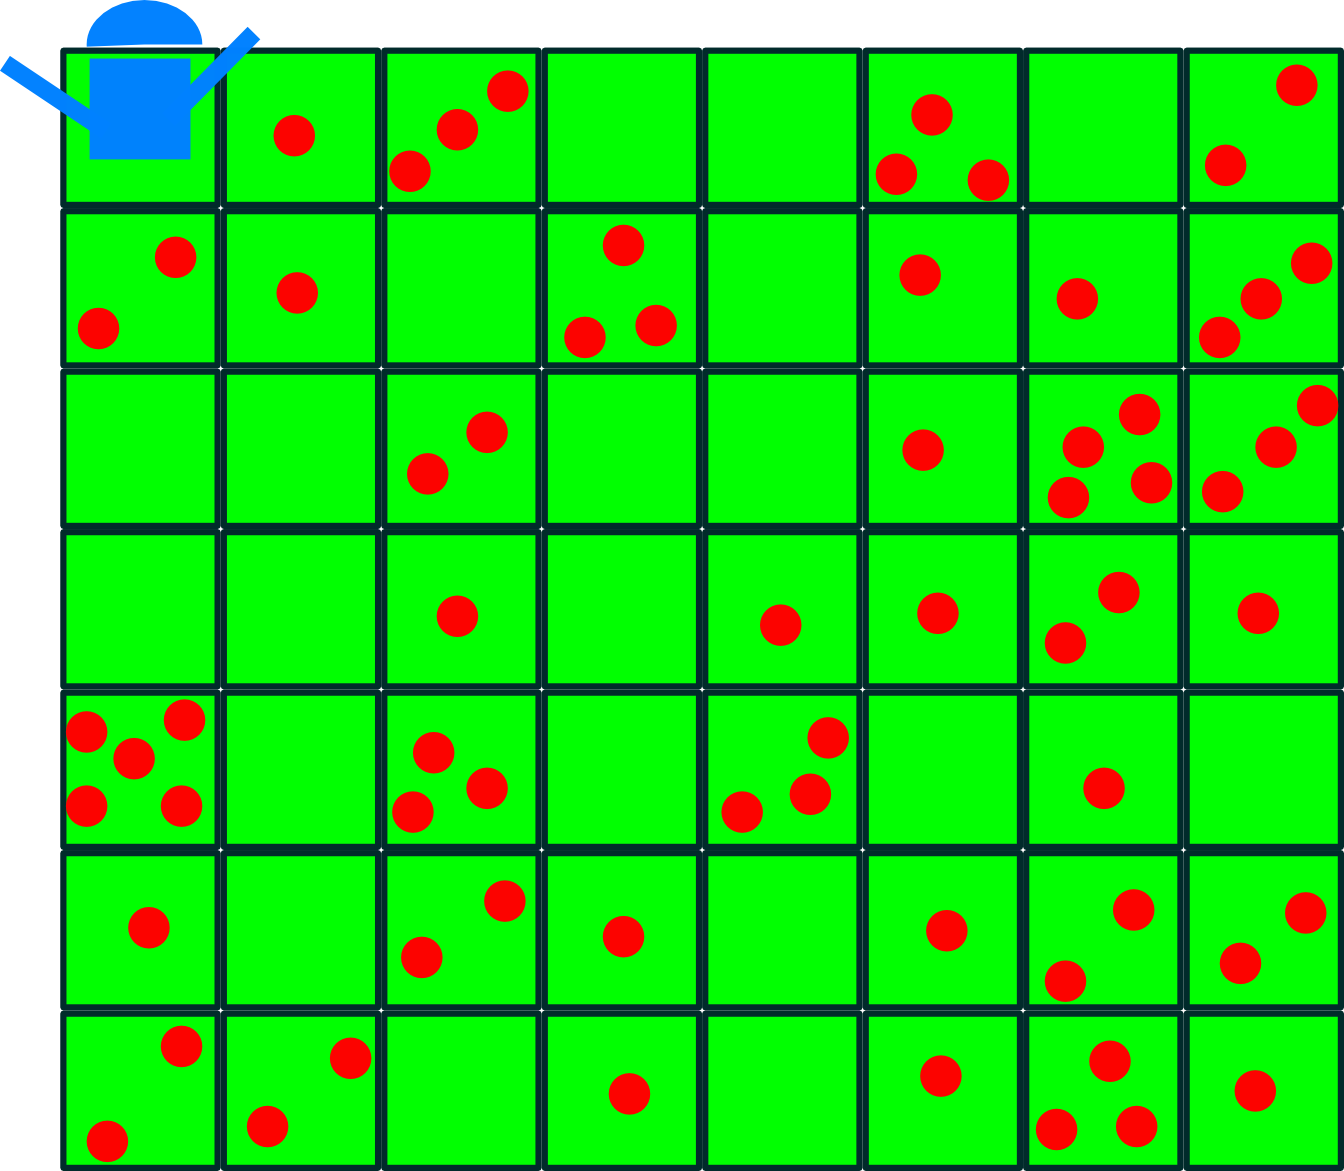
\includegraphics[width=0.5\textwidth]{../img/applefield}
  \end{center}
\end{frame}

\begin{frame}
  \frametitle{Example 2: Apple Field -- complete search}
  \begin{center}
    {\smaller One possible (non-optimal) solution}\\
    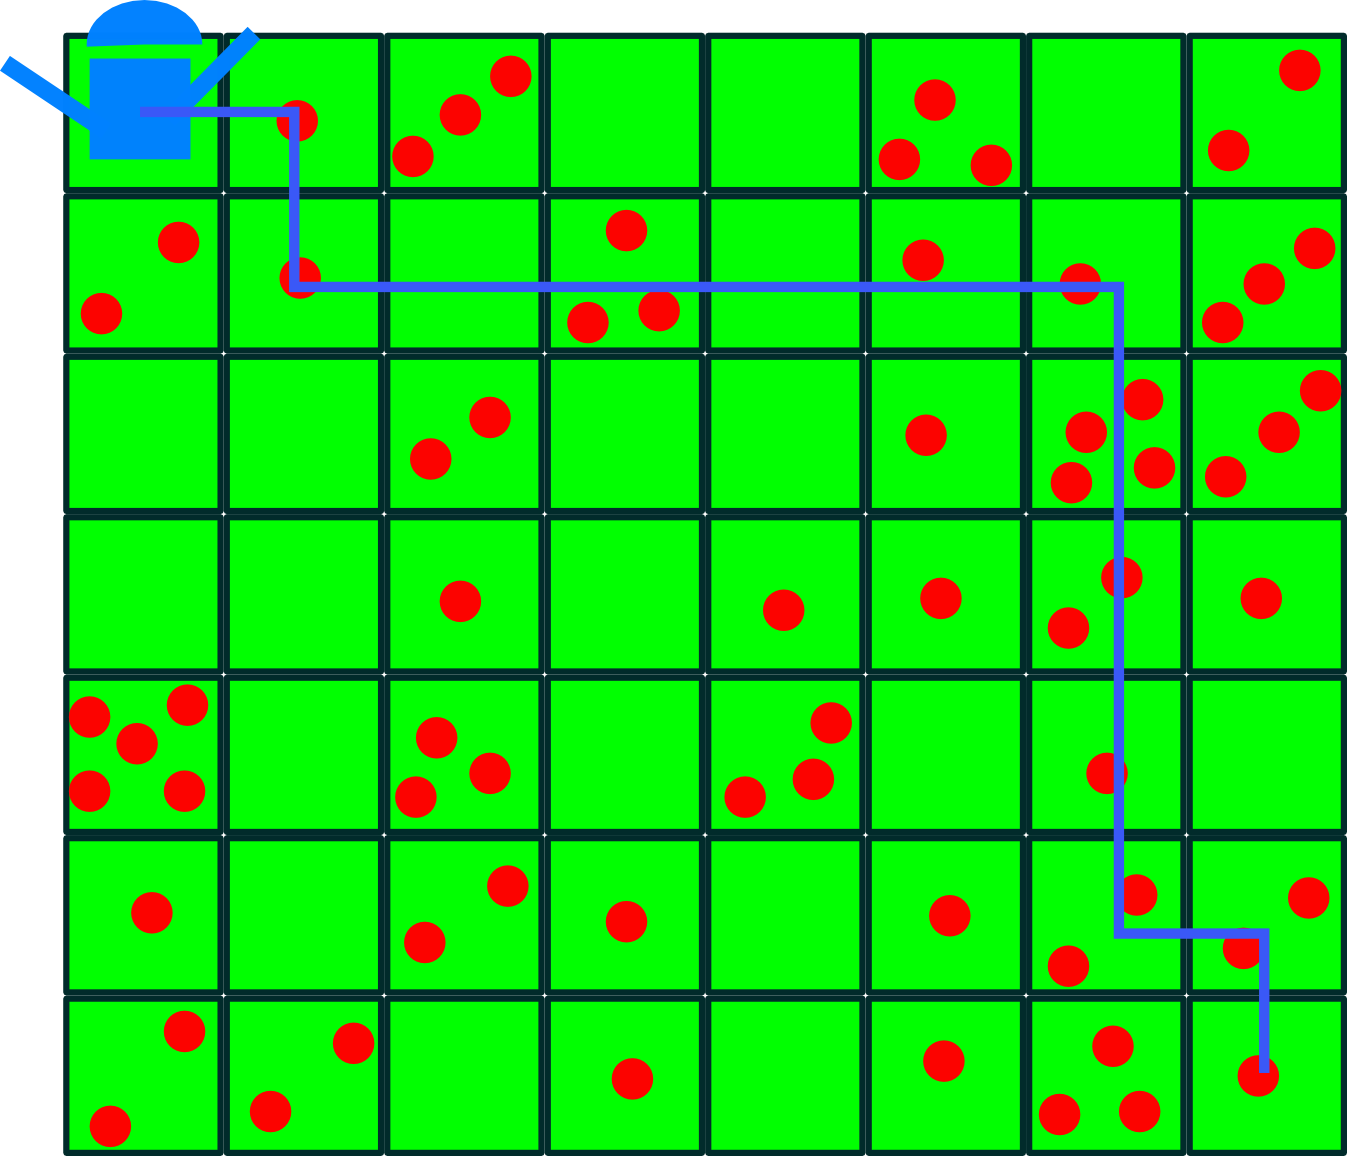
\includegraphics[width=0.5\textwidth]{../img/applefield-solution}
  \end{center}

  For every square, the robot can choose to go right (east) or down
  (south). How many possible paths exist?

  \bigskip

  And how many overlapping solutions are there?
\end{frame}

\begin{frame}
  \frametitle{Example 2: Apple Field -- overlapping solutions}
  \begin{center}
    {\smaller One possible (non-optimal) solution}\\
    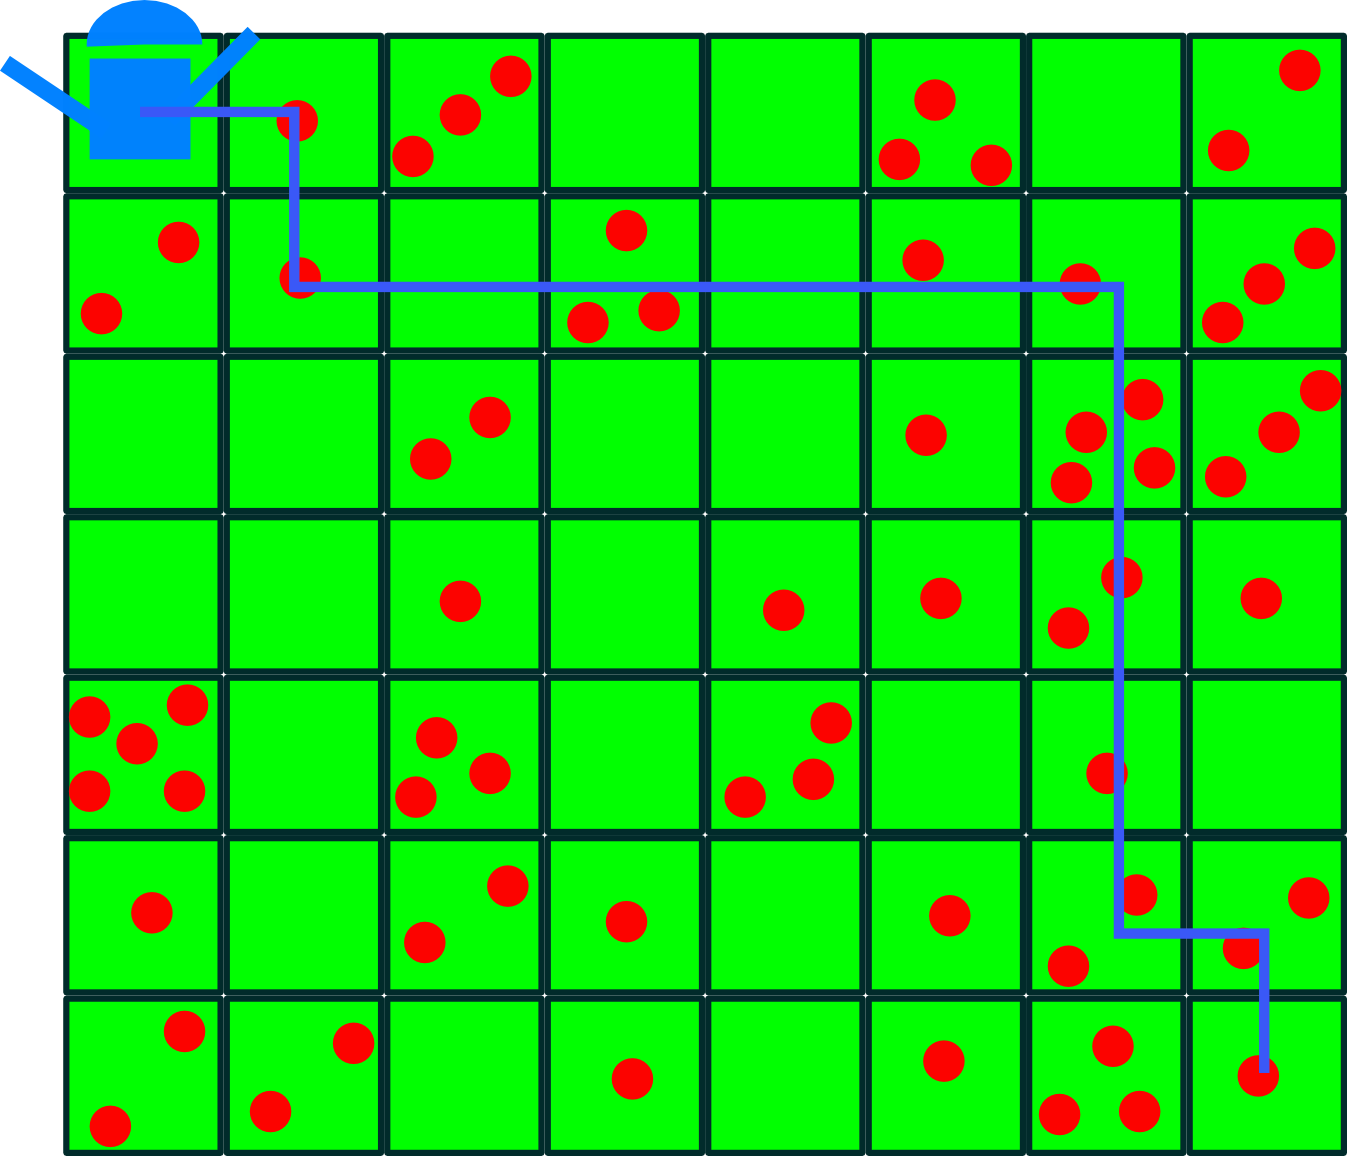
\includegraphics[width=0.5\textwidth]{../img/applefield-solution}
  \end{center}

  If the robot reached position (x,y) with k apples, it does not
  matter how it did it. So the path from (x,y) to the goal is independent from
  the parent path.

  This smells like DP! Let's solve it with a bottom up approach.
\end{frame}

\begin{frame}
  \frametitle{Example 2: Apple Field -- Bottom up DP}

  {\small
  \begin{itemize}
  \item \structure{tables:} We want to maximize the number of apples
    at the goal. Let's try a m*n position table. At each cell, we want
    to store the maximum number of apples achievable at that cell.

    \medskip

    We also want a second table, \emph{path}, which will store the path
    used.

    \vfill

  \item \structure{initial condition:} We can fill the top row (x,1) of the
    table with the sum of apples from 1 to x. And we can fill the Left column
    with the sum of apples from 1 to y.

    \medskip

    Alternatively, we can add an additional dummy ``-1'' column/line
    and fill it with zeros.

    \vfill

  \item \structure{transition:} For each cell x,y, max(x,y) is either
    max(x-1,y) + apple(x,y) or max(x,y-1) + apple(x,y)
  \end{itemize}}
\end{frame}

\begin{frame}[fragile]
  \frametitle{Example 2: Apple Field -- Let's see some code}
  {\smaller
  \begin{block}{}
\begin{verbatim}
// Assume apple[0,] and apple[,0] are all zeroes.
int apple[m][n]// Input.
int sum[m][n]// DP table, set to 0 using memset
int parent[m][n][2]// Path table, set to 0 using memset

for i in (1:m):
  for j in (1:n):
    sum[m][n] = apple[m][n] + max(sum[m][n-1],sum[m-1][n])
    if (sum[m][n-1] > sum[m-1][n]):
       parent[m][n][0] = m, parent[m][n][1] = n-1
    else:
       parent[m][n][0] = m-1, parent[m][n][1] = n
\end{verbatim}
\end{block}
  }
\end{frame}

\subsection{Flight Planner}
%%%%%%%%%%%%%
%% Example 2 -- UVA 10337 Flight Planner
% 1 Mile Altitude and 1(x100) miles distance
% wind speed map
% fuel cost: Climb +60, hold +30, sink +20 - windspeed wsp[alt][dis]
% Compute min fuel cost from (0,0) to (0,X=4)

%% First guess: Complete search/Backtracking finding path with minimal fuel cost
% Recurrence: minimum of current + climb/Hold/Dive
% Problem: 1000 distance columns: 3^1000 states to search!
% However, there are MANY overlapps: at any column/height, former path does not matter.

%% DP solution
% TOP down: create a 2D table and store computation value of subproblems as they are seen.
% Bottom-up: Start at 0 fuel used. Calculate next column based on where current column can reach
%            Bottom up hint: We just need to store two columns at a time (if only final result is desired)

\section{Classical DP}
\subsection{Max Sum}

\begin{frame}
  \frametitle{Classical DPs: 1D Range Sum}

  Given an array A containing $< 20K$ non-zero integers,
  \structure{determine the maximum range sum} of A.

  \begin{center}
    A = 1, -3, 20, -2, -5, 10, 5, -4, 6, 47, -30, -3\\
    S = -, --, \alert{20, -2, -5, 10, 5, -4, 6, 47}, ---, --
  \end{center}

  \vfill

  \begin{block}{What is a range sum?}
    A maximal range sum is two indexes $i,j, i < j$ in A that maximizes
    the sum $a_i + a_{i+1}, a_{i+2}, \ldots, a_j$.
  \end{block}
\end{frame}

\begin{frame}[fragile]
  \frametitle{Search Approaches for 1D Range Sum}
  \begin{block}{Naive Complete Search O($n^3$)}

    Naive approach: For every possible pair i,j, add the values
    between i and j and save the result.

{\smaller
\begin{verbatim}
maxindex = []
maxsum = 0
for i in (0:n):
   for j in (i:n):
      sum = 0
      for k in (i:j):
         sum += k
      if sum > maxsum:
         maxsum = sum
         maxindex = [i,j]
\end{verbatim}
}
  \end{block}
\end{frame}

\begin{frame}[fragile]
  \frametitle{Search Approaches for 1D Range Sum}
  \begin{block}{Better Complete Search -- $O(n^2)$}

    If we initialize A with the right values, we can skip the sum in
    the loop of the previous slide.

{\smaller
\begin{verbatim}
A = [], maxsum = 0
for (i in 0:n):
   A[i] = A[i-1] + input
   // A[i] now has the sum 0..i

for (i in 0:n):
   for (j in i:n):
      sum = A[j] - A[i-1]
      if sum > maxsum:
         maxsum = sum
         maxindex = [i,j]
\end{verbatim}
}
  \end{block}
\end{frame}

\begin{frame}
  \frametitle{Search Approaches for 1D Range Sum}
  Using the $O(n^2)$ pre-computation:

  \bigskip

  \begin{center}
    Input = 1, -3, 20, -2, -5, 10, 5, -4, 6, 47, -30, -3\\
    A = 1, -2, 18, 16, 11, 21, 26, 22, 28, 75, 45, 42\\
  \end{center}

  \bigskip

  \begin{itemize}
  \item Subset: 2 to 9 = A[9] - A[2-1] = 75 - (-2) = 77;
  \item Subset: 0 to 9 = A[9] - 0 = 75;
  \item Subset: 5 to 6 = A[6] - A[5-1] = 26 - 11 = 15;
  \end{itemize}

  \bigskip

  Can we do better?

\end{frame}

\begin{frame}[fragile]
  \frametitle{1D Sum -- Kadane's Greedy Algorithm}
  \begin{block}{Greedly Max Sum O(n)}
      {\smaller
\begin{verbatim}
A[] = { 4, -5, 4, -3, 4, 4, -4, 4, -5};
int sum = 0, ans = 0;
for (i in 0:n):
   sum += A[i], ans = max(ans, sum)
   if (sum < 0) sum = 0; // reset greedy
\end{verbatim}
      }
  \end{block}

\begin{itemize}
\item Sum is the answer if we sum all the numbers
\item Sum is reset to zero if we ever go negative\\
  (better to start again)
\item At each step, we have two choices: add the sum from the previous
  step, or start from zero.
\end{itemize}
\end{frame}

\subsection{Maximum 2D Sum}
\begin{frame}
  \frametitle{Classic DP -- Maximum 2D sum}
  \begin{block}{Problem Summary}
    Given an array of positive and negative numbrers, find the
    subarray with maximum sum.
  \end{block}

  \bigskip

  \begin{center}
    \begin{tabular}{|cccc|}
      \hline
      0 & -2 & -7 & 0\\
      9 & 2 & -6 & 2\\
      -4 & 1 & -4 & 1\\
      -1 & 8 & 0 & -2\\
      \hline
    \end{tabular}
  \end{center}

  \bigskip

  How big would be a complete search for this problem?
\end{frame}

\begin{frame}[fragile]
  \frametitle{Maximum 2D Sum -- Complete Search}

\begin{block}{}
  A complete search approach needs 6 loops (2 for each coordinate, 2
  for the sum), for a total complexity of O($n^6$).
\end{block}

\begin{block}{}
{\smaller
\begin{verbatim}
minvalue = -MIN_INT
for i in (0:n):
   for j in (0:n):
      for k in (i:n):
         for l in (j:n):
         sum = 0
         for a in (i:k):
            for b in (j:l):
               sum += A[a,b]
         if sum > minvalue:
            minvalue = sum
\end{verbatim}
}
\end{block}
\end{frame}

\begin{frame}[fragile]
  \frametitle{Max 2D sum using partial sums}
  \begin{block}{}
    The ``partial sum'' algorithm used for 1D arrays can also be
    adapted to 2D Matrices, using the ``inclusion/exclusion''
    principle.
  \end{block}

\begin{block}{}
{\smaller
\begin{verbatim}
for i in (0:n):
   for j in (0:n):
       A[i][j] = input
       if (i > 0) A[i][j] += A[i-1][j]
       if (j > 0) A[i][j] += A[i][j-1]
       // Avoid double count
       if (i > 0 && j > 0) A[i][j] -= A[i-1][j-1]

for i,j in (0:n)(0:n):
   for k,l in (i:n)(j:n):
      sum = A[k][l]
      if (i > 0) sum -= A[i - 1][l];
      if (j > 0) sum -= A[k][j-1];
      if (i > 0 && j > 0) sum += A[i-1][j-1]
      maxsum = max(sum,maxsum)
\end{verbatim}
}
\end{block}

\end{frame}

\subsection{Longest Increasing Subsequence}

\begin{frame}
  \frametitle{Classic DP: Longest Increasing Subsequence}
  \begin{block}{Problem Definition}
    Given a sequence $A = \{A[0],A[1],\ldots,A[n]\}$, determine the
    longest subsequence of increasing numbers.

    \smallskip

    Note that the numbers do not need to be contiguous.
  \end{block}

  Example:

  \bigskip

  A = \{ \alert{-7}, 10, 9, \alert{2}, \alert{3}, \alert{8}, 8, 1\}
\end{frame}

\begin{frame}[fragile]
  \frametitle{Longest Increasing Subsequence: Complete Search}

  The complete search for the LIS problem requires you to test
  all possible subsets. This takes $O(2^n)$.

  \bigskip

  Very slow for any $n$ big enough :-(

  {\small
  \begin{block}{}
    Remember that you can easily list all subsets using a loop on a bitmask:
    {\smaller
\begin{verbatim}

for (i in 0:1<<n):
   subset = []
   ind = 0
   while (1 << ind) < i:
      if (1 << ind) & i:
         subset.append(set[ind])
      ind++

   if len(subset) > maxlen:
      maxlen = len;
\end{verbatim}
    }
  \end{block}}
\end{frame}

\begin{frame}
  \frametitle{Longest Increasing Subsequence -- DP approach}
  {\smaller
  \begin{block}{1 -- What is the state space?}
    For each element $A[i]$, we just need to know what is the size of
    the maximum subsequence up to that element.

    \medskip

    The element at the end of that sequence is either $A[i]$, or an element
    before $A[i]$ with the same max sequence size.
  \end{block}

  \bigskip

  \begin{tabular}{|c|c|c|c|c|c|c|c|c|}
    \hline
    A[i] & -7 & 10 & 9 & 2 & 3 & 8 & 8 & 1\\
    \hline
    LIS[i] & 1 & 2 & 2 & 2 & 3 & 4 & 4 & 2\\
    \hline
  \end{tabular}

  \begin{block}{2 -- What is the state transition?}
    For every $A[i+1]$ we find k in $0:i$ that has the biggest
    LIS$[k]$ where $A[k] < A[i+1]$. LIS$[i+1] =$ LIS$[k] + 1$.
  \end{block}

  The complexity of this approach is $O(n^2)$
  }
\end{frame}

\begin{frame}[fragile]
  \frametitle{Longest Increasing Subsequence -- DP approach}
  \begin{block}{}
  {\small
\begin{verbatim}
LIS[0:n] = 1
parent[0:n] = -1
for i in (1:n):
   for j in (0:i):
      if (LIS[j] >= LIS[i]) && (A[j] < A[i]):
         LIS[i] = LIS[j] + 1
         parent[i] = j
\end{verbatim}
  }
  \end{block}

\vfill

\begin{block}{}
  There is also a $O(n\text{log}k)$ approach that uses greedy
  algorithm and binary search. I'll leave that one for you to study at home!
\end{block}
\end{frame}

\subsection{Knapsack problem}
\begin{frame}[fragile]
  \frametitle{Classic DP: 0-1 Knapsack Problem}
  {\smaller
  \begin{block}{Problem Definition -- also known as \emph{subset sum}}
    Given a set $A$ with $n$ elements. Each element has a value $V_i$
    and size $S_i$. Calculate the subset with maximum sum
    $V_{subset}$ and $S_{subset} \leq S$.
  \end{block}

  \medskip

  \begin{tabular}{|c|c|c|c|c|}
    \hline
    $V_i$ & 100 & 70 & 50 & 10\\
    \hline
    $S_i$ & 10 & 4 & 6 & 12\\
    \hline
  \end{tabular}

  \smallskip

  $S = 12$

  \begin{block}{Complete Search Recursive Solution -- Similar to Wedding Problem}
    Consider the recursive function \emph{value(id,size)}, where
    \emph{id} is the item we want to test, and \emph{size} is the size
    remaining in the backpack.

    \medskip

\begin{verbatim}
value(id,size):
   if size == 0, return 0 // bag is full
   if id == n, return 0 // checked all items
   if S[id] > size, return value(id+1,size) // too big
   return max(value(id+1,size),
              V[id] + value(id+1, size - S[id]))
\end{verbatim}
  \end{block}
  }
\end{frame}

\begin{frame}
  \frametitle{0-1 Knapsack Problem: DP Approaches}

  {\small
    We can easily modify the algorithm in the last slide to a Top-down
    DP.

    \bigskip

    \alert{Just be careful}: the size of the state table is: $nS$.\\
    If $S$ is too large ($>>1M$), this approach might be unfeasible.
  }
\end{frame}

\subsection{Coin Change}
\begin{frame}
  \frametitle{Classical DP -- The Coin Change Problem (CC)}
  \begin{block}{Problem Summary}
    Given a target value $V$, and a list $A$ of $n$ coin sizes, what
    is the minimum number of coins necessary to represent $V$? Assume
    unlimited supply of coins.
  \end{block}

  Example: $V = 7$,$A = \{1,3,4,5\}$\\
  \medskip
  One answer is $5+1+1$. The optimal answer is $4+3$

  \bigskip

  \begin{exampleblock}{Recurrence}
    The number of coins for value $V$ is 1 + the number of coins for
    value $V - $\emph{size of coin}.
  \end{exampleblock}
\end{frame}

\begin{frame}[fragile]
  \frametitle{Coin Change -- Complete Search Algorithm}
  {\smaller
  \begin{block}{Recursive Complete Search Again!}
\begin{verbatim}
change(value):
   if value == 0: return 0 // 0 coins for 0
   if value < 0: return INF // impossible result
   min = INF
   for i in (0:n):
      t = 1 + change(value - A[i])
      if (t < min): min = t
   return t
\end{verbatim}

\medskip

Can you see the many overlapping subproblems?
  \end{block}
\begin{itemize}
  \item By now you should know how to do the top-down DP from here;
  \item Can you modify the recurrence to show \structure{how many
    different ways} you can complete a value?\\
    (hint: complexity does not change);
  \item If you have many queries $V$, but with the same set of coins
    $A$, you don't need to clear the table.
\end{itemize}


  }
\end{frame}



%\subsection{Travelling Salesman Problem}
%\begin{frame}
%  \frametitle{Classical DP -- Travelling Salesman Problem}
%
%  We will talk about TSP with DP Next Class!
%\end{frame}

%%%%%%%%%%%%%%%%%%%%%%%%%%%%%%%
% Travelling Salesman Problem (bitmask again)
%% Travelling Salesman Problem (TSP)
% State: tsp(pos,bitmask)
% Transition:
%   Each visited city is a bit in the bitmask
%   - if every city has been visited: tsp(pos, 2^n -1) = dist[pos][0] (back to the start with 0 cities)
%   - Else, try visiting unvisited cities one by one
%   - tsp(pos,bitmask) = min (dist[pos][nxt] + tsp(nxt,bitmask|1<<nt))) for every nxt != pos,
%                                                                           and nxt not visited
%                                                                           bitmask & 1<<nxt == 0

\section{Conclusion}
\subsection{Conclusion}
\begin{frame}
   \frametitle{Summary}

   Dynamic Programming is a \structure{smart way to do complete
     search}, when a large part of the search space is overlapping.

   \begin{itemize}
   \item \alert{Top-down DP}: recursive complete search with memoization;
   \item \alert{Bottom-up DP}: state table with iterative completion recurrency;
   \end{itemize}

   \vfill

%   \begin{block}{Next Class (20/5, 23/5)}
%     \begin{itemize}
%     \item DP on non-classical problems
%     \item Relationship between DP and DAG
%     \item Other ``cool'' DP techniques.
%     \end{itemize}
%   \end{block}
\end{frame}

\begin{frame}
   \frametitle{Read more about DP}
   \begin{itemize}
      \item \url{http://people.csail.mit.edu/bdean/6.046/dp/}
      \item \url{http://community.topcoder.com/tc?module=Static&d1=tutorials&d2=dynProg}
   \end{itemize}
\end{frame}

\subsection{This Week's Problems}

\begin{frame}
  \frametitle{This Week's Problems}
  \begin{itemize}
  \item Dominator
  \item Forwarding Emails
  \item Ordering
  \item Place the Guards
  \item Doves and Bombs
  \item Come and Go
  \item ACM Contest and Blackout
  \item Ancient Messages
  \end{itemize}
\end{frame}

\begin{frame}
  \frametitle{Problem Hints (0)}

  {\smaller
  \begin{block}{Library!}
    For many of these problems, you will use a lot of repeated code:
    \begin{itemize}
    \item Visited Node arrays;
    \item Adjacent lists;
    \item Parent nodes;
    \end{itemize}

    \bigskip

    Prepare a template for the most common codes you use, and
    copy-paste it whenever necessary!
  \end{block}
  \begin{block}{Tricky Cases}
    \begin{itemize}
    \item Graphs with 1 or 0 Vertex
    \item Unconnected Graphs
    \item Self Loops
    \item Double edges
    \end{itemize}
  \end{block}
  }
\end{frame}

\begin{frame}
  \frametitle{Problem Hints (1)}  
  {\smaller
    \begin{block}{Dominator}
      \begin{itemize}
        \item If All paths from 0 to node B pass through node A, then node A {\bf dominates} node B;
        \item For all pair of nodes $i,j$, output ``Y'' if $i$ {\bf dominates} $j$, or ``N'' if not;
      \end{itemize}
    \end{block}

    \bigskip

    The idea of this problem is one of ``reachability'' -- can I reach
    node $j$ if I remove node $i$ from the graph?

    \bigskip

    Note: if $j$ is not connected to ``0'', then \emph{no one dominates j}
  }
\end{frame}

\begin{frame}
  \frametitle{Problem Hints (2)}
  {\smaller
    \begin{block}{Forwarding Emails}
      Every person $i$ sends e-mail only to person $j$.
      
      \bigskip
      
      What is the longest email chain?
      
      \bigskip
      
      Where does it start?
    \end{block}
    
    \begin{itemize}
    \item How do you deal with loops?
    \item Time limit is not very large, Try to find an O(n) solution!
    \end{itemize} 
  }
\end{frame}

\begin{frame}
  \frametitle{Problem Hints (3)}
  {\smaller
    \begin{block}{Ordering}
      Print all possible Orderings of a Direct Acyclic Graph

      \bigskip

      Generalize the DAG ordering algorithm which we discussed in class.
    \end{block}
    
    \begin{block}{Palace Guards}
      \begin{itemize}
        \item How do you represent the roads and junctions as a Graph?
        \item Find a ``guard-no guard'' assignment to vertices of the
          graph.
        \item First test if a solution is possible!
      \end{itemize}
    \end{block}    
  }
\end{frame}

\begin{frame}
  \frametitle{Problem Hints (4)}
  {\smaller
    \begin{block}{Doves and Bombs}
      This problem is about finding ``critical vertices'' in a
      graph. But how do you calculate the ``pigeon value'' of a
      vertex?
    \end{block}

    \begin{block}{Come and Go}
      Straight implementation of ``Strong Connected Components''. Be
      careful with tricky graphs!
    \end{block}    
  }
\end{frame}

\begin{frame}
  \frametitle{Problem Hints (5)}
  {\smaller
    \begin{block}{ACM Contest and Blackout}
      Goal: Find the {\bf First} minimum spanning Tree and the {\bf
        Second} minimum spanning Tree
    \end{block}

    \bigskip
    
    \begin{itemize}
    \item In this class we discussed how to find the Minimum Spanning Tree      
    \item How would we find the {\bf second minimum?}
    \item Idea: Maybe if we remove some edges from the graph?
    \end{itemize}
  }
\end{frame}

\begin{frame}
  \frametitle{Problem Hints (6)}
  \begin{block}{Ancient Message -- Challenge problem!}
    Count the symbols inside an image -- order does not matter!

    \bigskip

    What is the {\bf Main} difference between the symbols?
  \end{block}
    
  \begin{itemize}
  \item The shape and size of the symbols is actually not important!
  \item Before you begin programming, discover what is the real
    difference between the symbols.
  \item Hint: The numbers ``1'', ``0'', ``8'' have the same difference.
  \end{itemize}    
\end{frame}


\end{document}

%\subsection{Extra}
%\begin{frame}
%  \frametitle{Extra -- ICPC Call to Arms!}

%  {\smaller
%  If you can solve complete search and DP problems quickly, \alert{you
%  probably can reach top 50\%} at the ICPC first round. Why not try it this year?
%
%  \begin{block}{ICPC team registration -- Deadline 06/10 -- Contest 06/23}
%    Send message to caranha@cs.tsukuba.ac.jp with the following information:
%    \begin{itemize}
%    \item Team Name -- roman letters, numbers and symbols
%    \item Team Member 1 -- Name (letters), Name (japanese), e-mail, student ID
%    \item Team Member 2 -- Name (letters), Name (japanese), e-mail, student ID
%    \item Team Member 3 -- Name (letters), Name (japanese), e-mail, student ID
%    \end{itemize}
%  \end{block}}


%  {\tiny
%  \begin{itemize}
%  \item Japan 1st Round contest 2011 --\\
%    \url{http://ichyo.jp/aoj-icpc/?source4=0&source2=0&source3=0&source1=1&year_max=2011&year_min=2011}
%  \item Japan 1st Round contest 2012 --\\
%    \url{http://ichyo.jp/aoj-icpc/?source4=0&source2=0&source3=0&source1=1&year_max=2012&year_min=2012}
%  \item Japan 1st Round contest 2013 --\\
%    \url{http://ichyo.jp/aoj-icpc/?source4=0&source2=0&source3=0&source1=1&year_max=2013&year_min=2013}
%  \item Japan 1st Round contest 2014 --\\
%    \url{http://ichyo.jp/aoj-icpc/?source4=0&source2=0&source3=0&source1=1&year_max=2014&year_min=2014}
%  \end{itemize}}
%\end{frame}
%\end{document}
